\subsection{Explicaci\'on del algoritmo}
La metaheurística de Búsqueda Tabú, se basa en una heurística de Búsqueda Local y permite escapar de los óptimos locales para intentar encontrar mejores soluciones. Incorpora estructuras de memoria para llevar un registro que permite elegir vecindades evitando aquellas que ya fueron visitadas (de esta manera no se forman ciclos). Esta estructura es llamada lista Tabú, debemos definir que información de las soluciones que visitamos va a almacenar y en qué medida.

En nuestro algoritmo para implementar la lista Tabú primero pensamos en guardar las soluciones que iban surgiendo, pero fue descartada porque el número de soluciones que visitamos puede ser muy grande, si pensamos en que las cliques son conjuntos de nodos, entonces se podrían formar muchas combinaciones que tendremos que evaluar al momento de obtener un candidato.
Finalmente nos decantamos por almacenar nodos visitados, que nos permite acotar la lista en el número de nodos del grafo. Un nodo ingresa a la lista Tabú si fue apartado de la solución en el movimiento de una solución a una vecina. 

Por medio de un esquema podemos mostrar el funcionamiento de la metaheurística:
\begin{center}
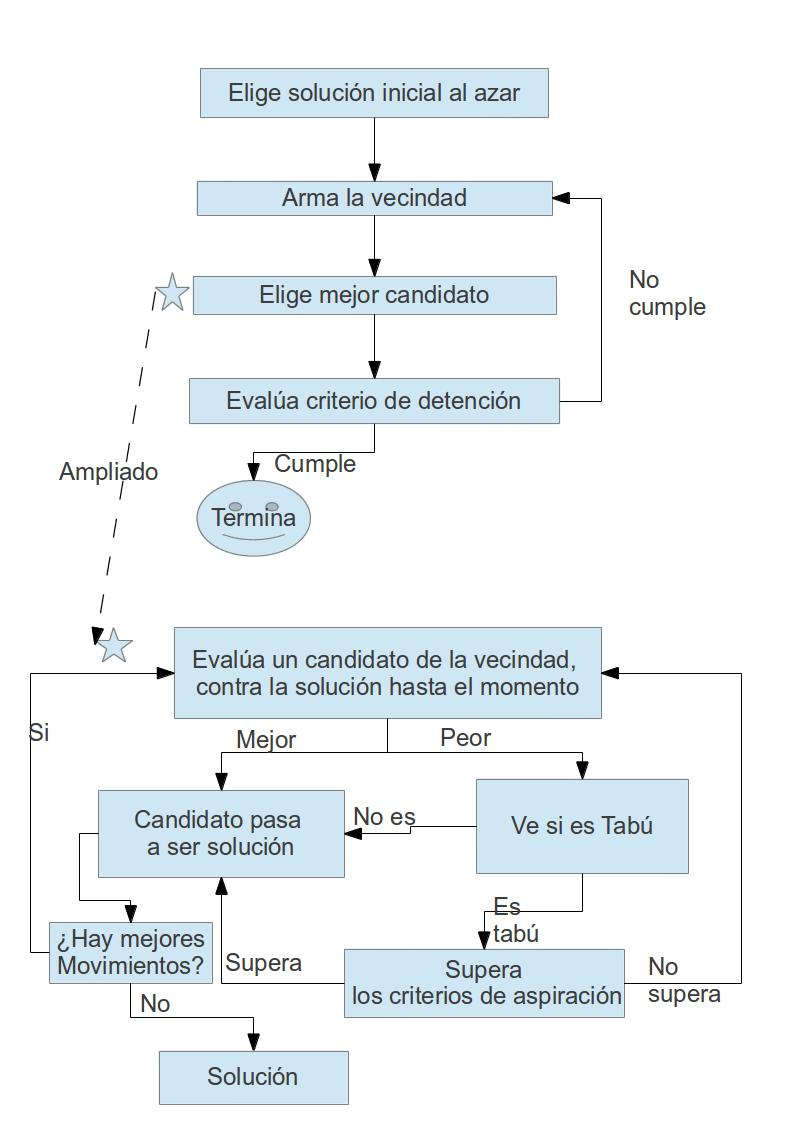
\includegraphics[scale=0.3]{tabu/esquema.jpg}
\end{center}

\subsection{Pseudoc\'odigo y complejidad}
\begin{algorithm}
	\caption{Tabú Search}\label{tabu}
	\begin{algorithmic}[1]
	\Procedure{Tabu }{$G\ =\ (V,\ E)$}
		\State $CMF=\ random(nodos)$	\Comment{elige un nodo al azar}
		\State $Clique=\ CMF$
		\State $lista_tabu=\ vacio$
		\While{$nro\_iteraciones\ \leq\ |E|$}
			\State $armar\_vecindad(Clique)$
			\ForAll{$vecino\ in\ vecindad$}
				\If{$frontera(vecino)\ >\ frontera(CMF)$} \Comment{si es mejor que la mejor solución hasta el momento lo cambia sin importar si es tabú}
					\State $CMF=\ vecino$
					\State $Clique=\ CMF$ 
					\State $Actualizar\_lista\_tabu$
				\EndIf
			\EndFor
		\EndWhile

		\If{$CMF\ no\ cambio$}
			\If{$\exists \ vecino\_no\_tabu$}
				\State $Clique=\ vecino\_no\_tabu$
				\State $Actualizar\_lista\_tabu$
			\Else
				\State $Clique=\ algun\_vecino$
			\EndIf
		\EndIf
	\EndProcedure
\end{algorithmic}
\end{algorithm}


\subsection{Casos nefastos}


%\subsection{Experimentaci\'on}




